\chapter{Age pattern models}
\label{theory-age_pattern_model}
The compartmental model of process in the previous section leaves one
part unspecified: how should the age-specific rates be modeled?  In
this section, I develop the mathematical and statistical theory behind
a model for age specificity in epidemiological rates, such as
incidence, remission, without-condition mortality, and
excess-mortality rates.

\begin{figure}[h]
\begin{center}
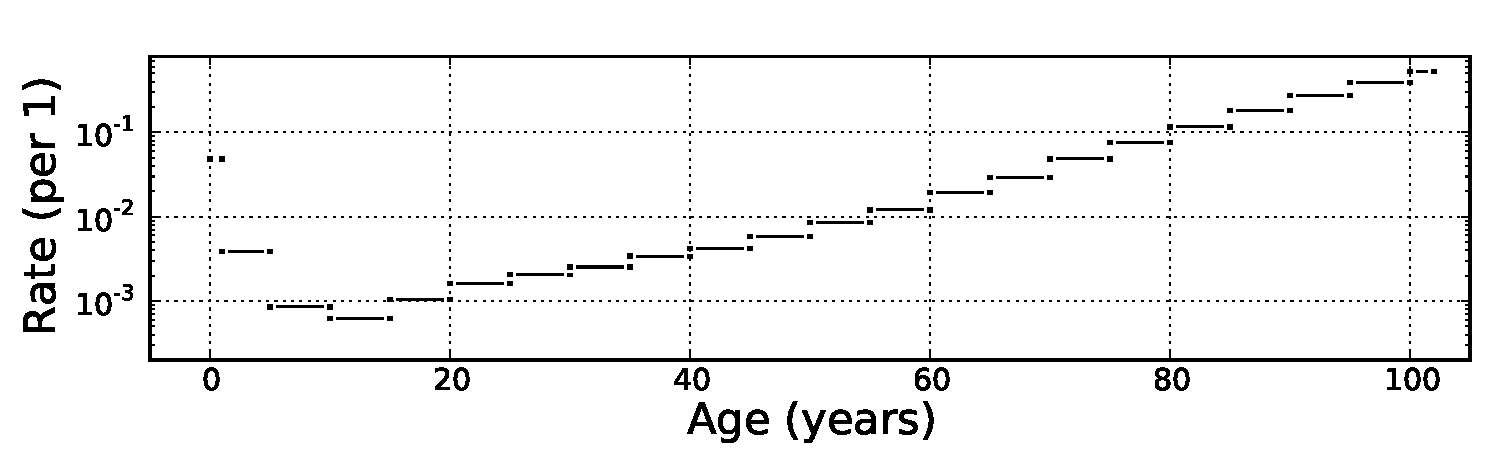
\includegraphics[width=\textwidth]{ssas-mx_female_1990.pdf}
\caption{All-cause mortality for females in the sub-Saharan Africa,
  Southern region in 1990 as a function of age shows the range of
  variation in age-specific rates.  $m_{\all}$ is as low as 6 per
  10,000 PY at age 10, but rises to 5,000 per 10,000 PY at age 100.}
\label{ssas-mx_female_1990}
\end{center}
\end{figure}

Epidemiological rates vary between regions, times, and sexes as well
as age.  A figure like Figure~\ref{ssas-mx_female_1990} for the Asia
Pacific, High Income region in 1990 would look very different, as
would the sub-Saharan Africa, Southern region in 2010. However,
systematic variation as a function of \emph{age} is often the largest
source of variation by orders of magnitude, and furthermore, this
variation is not linear.

The approach that I have taken for modeling age-specific rates draws
on the mathematical theory of spline interpolation, and the
statistical theory of smoothing splines.

\section{Introduction to Spline Models}

Although I consider the spline model part of the ``model of process''
in the integrative systems modeling dichotomy, it is most instructive
to develop it from a foundation in the statistical technique of linear
regression, which makes it appear closer to a model of data.

As motivation for our discussion around flexible modeling of
continuous variables, consider this simple model relating the
conditional mean of some variable $Y$ to a continuous predictor
$X$ 
\[
E[Y \mid X] = f(X),
\]
where $f(X)$ is some function of $X$. In the case where $f(X) =
\beta_0 + \beta_1 X$, we see that this model returns the familiar form
of a linear regression of $Y$ on $X$.

In many cases, the relationship between the conditional mean of $Y$
and $X$ is nonlinear (see, for example, the data depicted in
Figure~\ref{ssas-mx_female_1990}). It is common to address this sort
of nonlinearity by including higher order polynomial transformations
of the variable $X$ to capture potential nonlinearity. For example, we
could augment the simple linear regression above with $X^2$ and $X^3$
terms to represent the relationship as a third degree
polynomial 
\[
E[Y|X] = \beta_0 + \beta_1 X + \beta_2 X^2 + \beta_3 X^3.
\]
While this model can capture a nonlinear relationship between $X$ and
$Y$, it is limited to that which can be represented as a cubic
polynomial.  In statistical practice, it is often found that
polynomial approximations of this type can have erratic behavior at
the boundaries of the observed data \cite{ESL}. Furthermore,
polynomial regressions may lack the necessary flexibility to capture
complex non-linear relationships. As such, a more flexible solution
with better behavior is needed.

In both of the above mentioned cases, the functional form of $f(X)$
can be expressed as follows:
\[
f(X) = \sum_{i=0}^m\beta_m h_m(X),
\]
where $h_i(X)$ is the $m^{th}$ transformation of the variable $X$. For
example, we see that \begin{itemize} \item if $f(X) = \beta_0 +
  \beta_1 X$, $h_0(X)=1$ and $h_1(X) = X$, and \item if $f(X) =
  \beta_0 + \beta_1 X + \beta_2 X^2 + \beta_3 X^3$, $h_0(X) = 1$, and
  $h_i(X) = X^i$, for $i=1,2,3$. \end{itemize} The functions $h_i$
represent a linear basis expansion of the variable $X$, and serve to
motivate our discussion around flexible modeling.

Models represented in this way are particularly attractive in that
they can be fit using any standard statistical software. One need only
provide the set of basis functions or data transformations and
estimate the parameters $\beta_i, i=0, M$ using least squares. Namely,
we can estimate the regression coefficients, $\beta_m,\; m=0, \dots,
M$, for our linear basis functions by minimizing 
\[
\sum_{i=1}^n\left(Y_i - \sum_{m=0}^M \beta_mh_m(X_i)\right)^2.
\]

\section{Definition of Splines Models}

\emph{Regression splines} or \emph{piecewise polynomials} refer to a
family of models which result from specific definitions of the basis
functions, $h_i$. These models arise by partitioning the variable $X$
into $k+1$ contiguous intervals at \emph{knot locations} $\xi_1,
\dots, \xi_{k}$. The function $f$ is then represented by different
polynomials in each interval. The simplest example of this is the
representation of $f$ as piecewise constant. In this case, we
have 
\[
h_0(X) = I(X \leq \xi_1),\; h_1(X)=I(\xi_1 < X \leq \xi_2), \;
\dots, h_{k}(X) = I(X > \xi_k). 
\]
As we see in Figure~\ref{splines_fig}, the resulting fit is a series
of horizontal (constant) lines in each of the specified intervals. In
particular, we see that in the $m^{th}$ interval, $\hat{\beta}_m =
\bar{Y}_m$, or the mean value of $Y$ in that interval.

A more favorable and flexible fit to the data might be achieved by
instead representing the data in each interval as a line, i.e. fitting
a piecewise linear model to the data. This can be achieved by the
following basis, 
\[
h_0(X) = 1,\; h_1(X) = X,\; h_2(X) = (X-\xi_1)_+,\; \dots,\; h_{k+2}=(X-\xi_k)_+,
\]
where the notation $h_+$ indicates the positive part of $h$. Models
fit using bases of this type are continuous but not differentiable at
the knot locations, as seen in Figure \ref{splines_fig}. In many
cases, a piecewise linear fit of this type is sufficient to capture
any non-linearity in the data, and this will be the typical model for
epidemiological rates in the second half of this book. However, a
popular alternative which yields ``smooth'' curves to the data are
piecewise cubic polynomials. These types of regression splines ensure
first and second order differentiability at the knot locations and
yield aesthetically pleasing fits at the expense of more parameters.


\begin{figure}[h]
\begin{center}
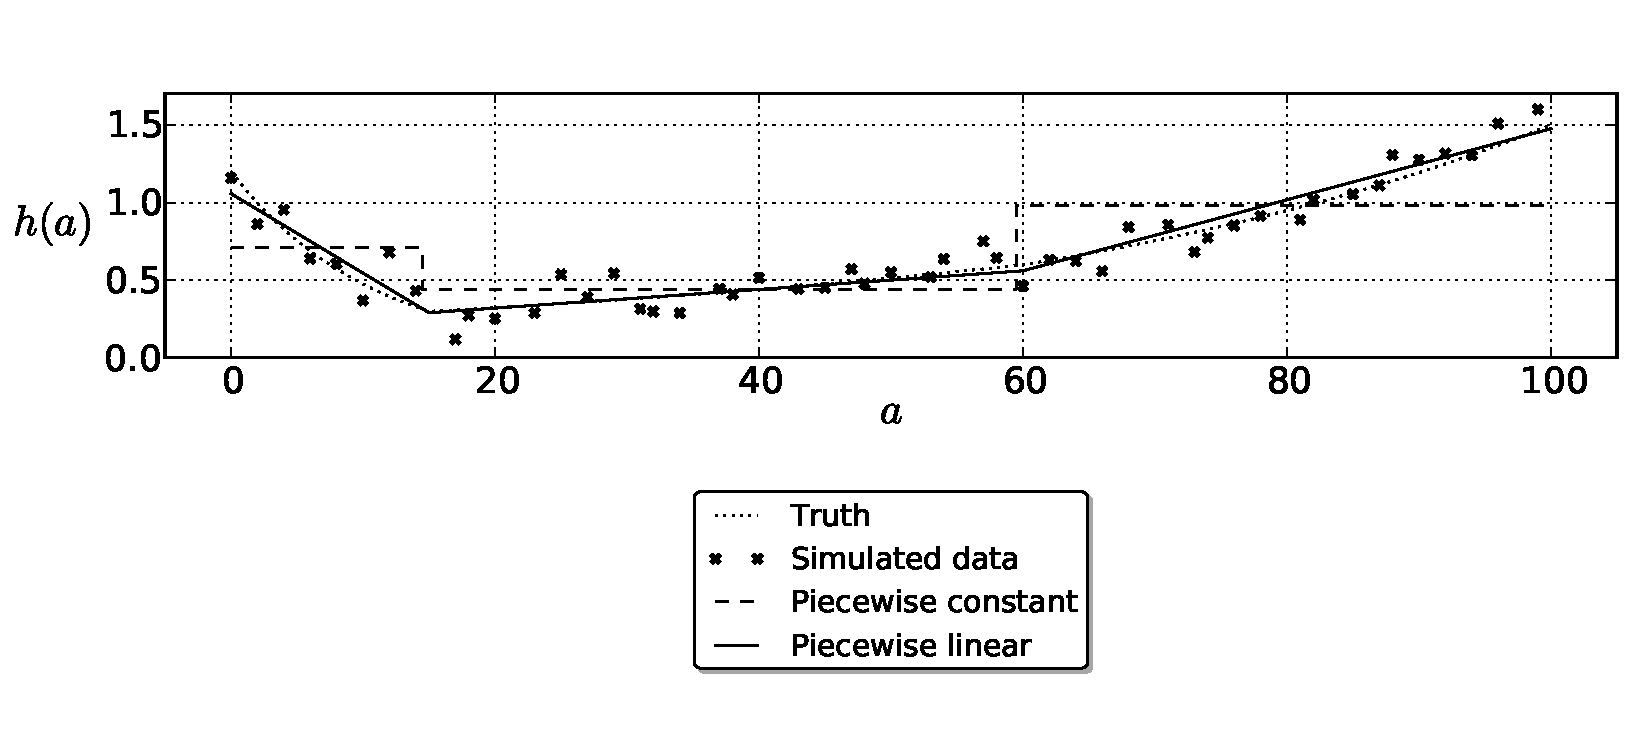
\includegraphics[width=\textwidth]{splines-fig.pdf}
\caption{Spline interpolation of simulated data. The true age-specific
  rate is piecewise log-linear, so none of the splines can represent
  it perfectly. The true age-specific rate and the models all have
  knot set $\{0, 15, 60, 100\}$.}
\label{splines_fig}
\end{center}
\end{figure}

We note that piecewise polynomial splines provide a useful tool for
flexible modeling of non-linear trends. However, it should also be
said that piecewise polynomial regressions tend to have the same
issues as polynomial regressions at the boundaries of the data. One
solution to this issue is to require that the fit is \emph{linear}
beyond the range of the data. Imposing these constraints results in
the \emph{natural spline}. The benefit of using natural splines is
that the imposed constraints yield two extra free parameters, which
can perhaps be more efficiently used by selecting two more interior
knots. Thus, the natural spline allows for more potential interior
flexibility of your fit with the same level of model complexity as its
piecewise polynomial counterpart.

Spline modeling has a long history, and a vast literature exists in
this area, including a wide exploration of various types of basis
expansions. We do not delve into this discussion further and refer the
reader to other more extensive treatments of the subject
\cite{Wahba_Spline_1990,ESL}.

\section{Choosing Knots}

To this point, we have taken for granted the choice of number and
location of the so-called ``knots'' in our model. However, as one
might imagine, this is not always a trivial task. Depending on the
data, the ``knots'' can have almost as much influence on the fit as
the choice of basis functions.

For the purpose of generic disease modeling, we advocate for an
informed choice of knot locations. Namely, knot locations should be
chosen \emph{a priori} to reflect expert knowledge about the disease
of interest and its behavior as a function of some continuous
variable. For example, in a recent study looking at global trends in
mean systolic blood pressure as a function of age, Danaei \emph{et al}
elected to use a cubic regression spline with knots located at ages 30
and 60 ($\xi_1 = 30$ and $\xi_2=60$) \cite{Danaei_National_2011}. These
choices reflect the expectation, based on literature and prior
knowledge, that the behavior of mean systolic blood pressure as a
function of age would be distinct in these intervals due to a) low
blood pressure in young adults, and b) survivor effects in elderly
populations.

Although this approach of using expert knowledge to inform the number
of knots and knot locations is practical and allows for users to
determine critical features of the model, it is certainly not the only
approach. Much literature is devoted to the choice of knot locations
and the number of knots. We refer our readers to \cite{ESL,
  Wand2001[KP2]} for further discussion of this topic.

An interesting direction for future work is to remove the requirement
for expert knowledge to inform knot selection.  This could proceed
through model selection or model averaging of models with a variety of
knot locations \cite{[ref baysian model averaging[KP3]]}, or through
techniques developed in the adaptive regression spline literature
\cite{[ref[KP4]]}, or by leaving spline models altogether and using Gaussian
processes or some similar non-parametric model for the age-pattern
\cite{[ref GP[KP5]]}.

\section{Smoothing Splines}
One approach to address the challenge of knot selection is to use
smoothing splines.  The smoothing spline can be formulated in a
Bayesian framework in terms of a prior representing the belief that in
the absence of evidence, the age-pattern is not varying.
Mathematically, this takes the form of a penalty on the root mean
square of the derivative of the age-specific rate $f$:
\[
\left(\int _{a=a_0} ^{a_1} \| f'(a) \|^2 dw(a)\right)^{1/2} \sim N(0, \sigma^2).
\]

For the piecewise linear smoothing splines that will be used most
frequently in the second half of this book, the derivative of $f$ is
constant between knots, so with equal weighting for smoothing at all
ages, the integral above simplifies to the following:
\[
\int _{a=a_0} ^{a_1} \| f'(a) \|^2 = \sum_{i=0} ^K \bigg(\sum_{j=1} ^{k-1} \beta_j\bigg)^2(k_{i+1}-k_i) / (k_K - k_0)
\]
Figure~\ref{smoothing-splines} shows the effect of increasing the
smoothing parameter $\sigma$.

\begin{figure}[h]
\begin{center}
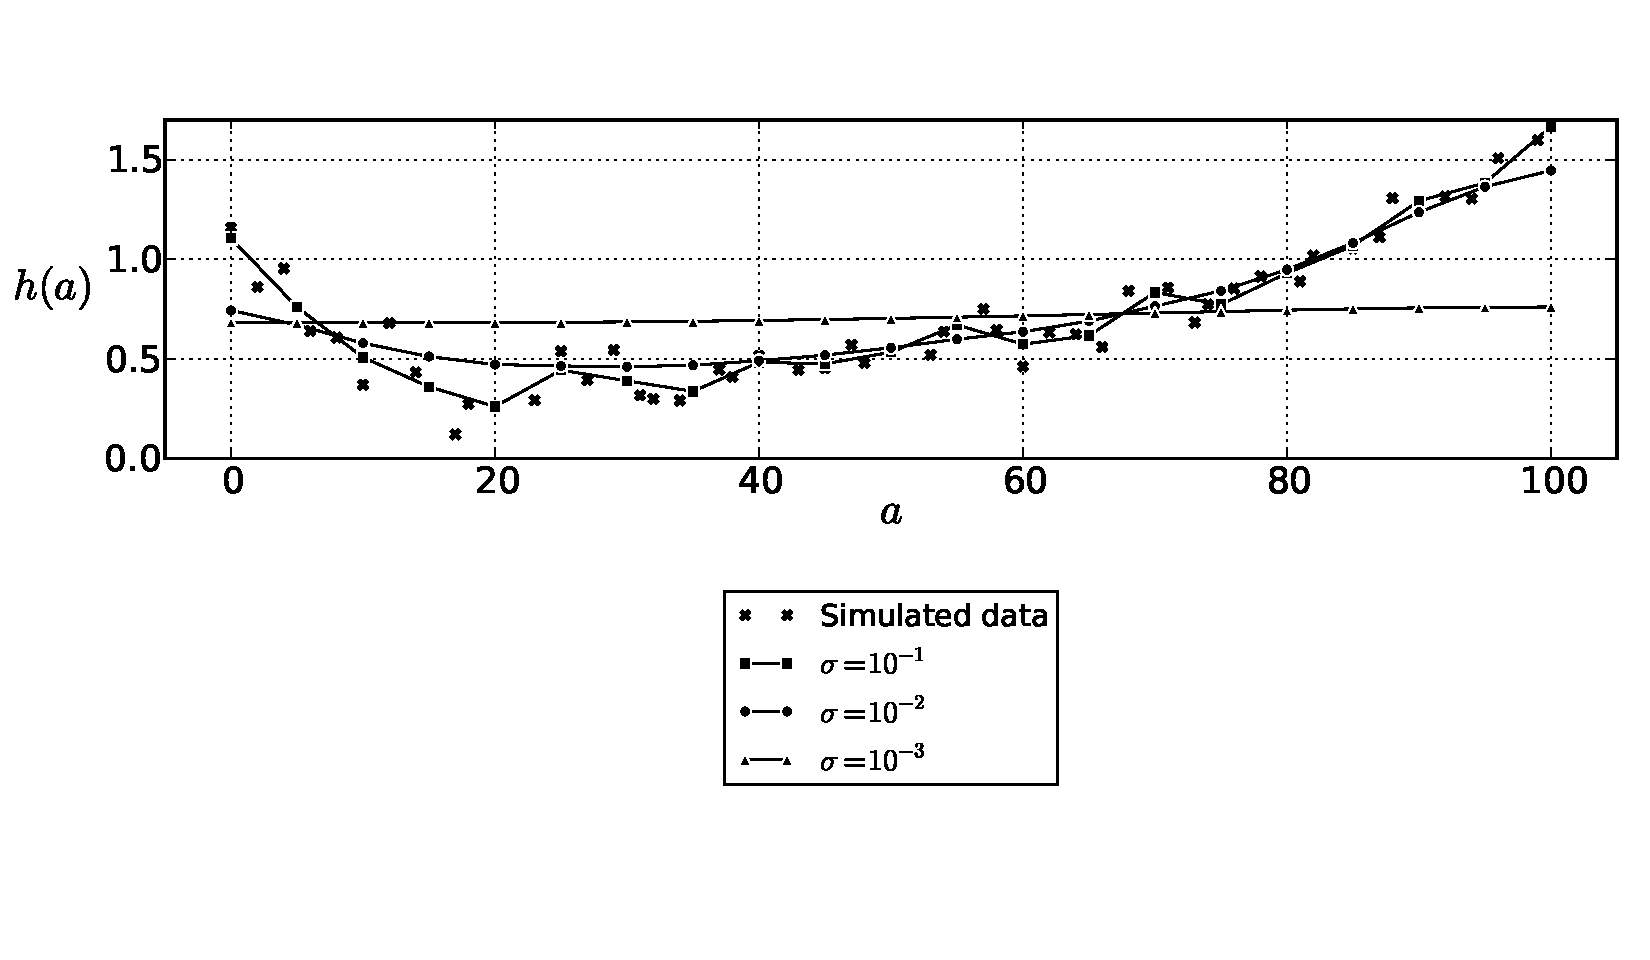
\includegraphics[width=\textwidth]{smoothing-splines.pdf}
\caption{Smoothing splines provide a solution to the challenge of knot
  selection in spline modeling.  Without smoothing, including many
  knots leads to estimates that are overly uncertain and wiggly.
  Smoothing, in the form of a quadratic penalty on the derivative of
  the age pattern, allows many knots to be included.}
\label{smoothing-splines}
\end{center}
\end{figure}


\section{Augmenting the spline model}
There are a few ways to augment the spline model that are useful when
modeling age-specific rates. Since the rates in the compartmental
model are always non-negative, I have parameterized the spline in
terms of the log of the knot values:
\[
\gamma_i = \log\bigg(\sum_{j=0}^I \beta_i\bigg).
\]
In order to fit the model in a Bayesian framework, I have defaulted to
giving these $\gamma_i$'s ``weakly informative'' priors,
\[
\gamma_i \sim \Normal\left(0, 10^2\right).
\]
This has very little effect on the posterior distribution, but makes
the prior ``proper'' and also helps with algorithm convergence in
some instances. In instances where relevant expert knowledge is
available, I can replace this with a more informative prior (this idea
is elaborated in the following section).

Finally, in order to deal with the order-of-magnitude differences of
age-specific rates, I have applied the spline smoothing to the
log-rate, rather than the rate itself.  This creates an additional
complication, however, because the informative priors often say that
rates are zero for certain ages.  In order to avoid the ill effects of
smoothing when the log-rate contains values of $-\infty$, I have
rounded up any $\gamma_i$ values that are below ten times the mean
rate.

TK smoothing in log-space.

TK smoothing and zeros.



Taken all together, the age-pattern model that will be used in this
book is then:
\begin{align*}
f(a) &= \sum_{i=0}^{K-1} 1[k_i <= a < k_{i+1}]\left( \frac{a-k_i}{k_{i+1}-k_i} e^{\gamma_i} + \frac{k_{i+1}-a}{k_{i+1}-k_i} e^{\gamma_{i+1}}\right),\\
\gamma_i &\sim \Normal\left(0, 10^2\right),\\
\widetilde{\|f'\|} &\sim \Normal(0, \sigma^2),\\
\end{align*}
where the integral of the derivative is approximated by
\[
\widetilde{\|f'\|} = \sum_{i=0}^{K-1}(\min(\gamma_i, \bar\gamma/10) -
\min(\gamma_{i+1}, \bar\gamma/10))^2/(k_K-k_0),
\]
and $\bar\gamma =
\sum_{i=0}^K \gamma/K$ and $\sigma$ is a model parameter that will
receive an informative expert prior.




\chapter{Expert priors on age patterns}

When dealing with sparse and noisy data, it is sometimes necessary to
include additional expert knowledge on the age pattern of
epidemiological rates.  For example, data sparsity can take the form
of a lack of information about rates of disease in children.  In
diseases where this is very rare, the fact that incidence is
effectively zero before a certain age is known by disease experts but
not represented in systematic review data.

A benefit of the Bayesian methods that will be used to fit the
integrative systems model is the conceptual and practical simplicity
of adding additional information to the age-pattern model.  This is
implemented by choosing a more informative prior distribution.  For
example, if the epidemiology of a disease is such that the incidence
level must be zero before age $a$, this can be incorporated by
replacing the weakly informative prior by the conditional probability
density with this constraint included.

There are three classes of additional information that will come up
frequently in the applications later in this book: level bound priors,
level value priors, and monotonicity priors. This section describes
how each can be implemented as an informative prior on the age pattern
model.


\section{Priors on level}

Informative priors on the level of the age pattern seem simple at
first, but may have unintended effects.  A prior on the level value
for certain ages says precisely that the age pattern should have that
value for those ages.  For example, Figure~\ref{level-value-priors} shows
the effects of adding a prior that the rate has value 0.1, 0.5, or 1.0
from age 0 to 15.


\begin{figure}[h]
\begin{center}
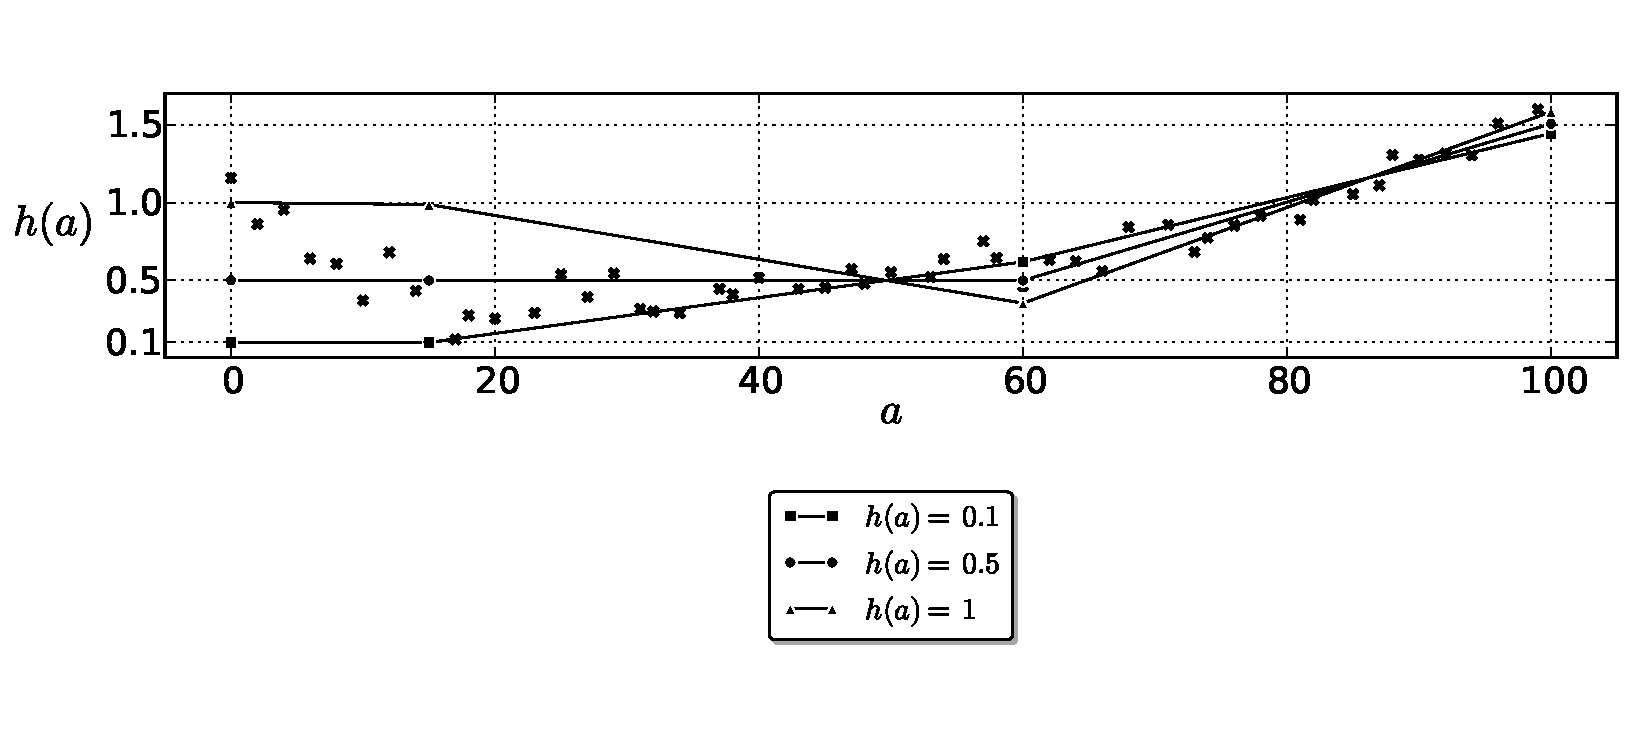
\includegraphics[width=\textwidth]{level_value-smoothing-splines.pdf}
\caption{An informative prior on the level of
$\mu(a)$ for $0 \leq a < 15$ changes the estimated rate dramatically
for $a$ between $20$ and $60$, and even leads to different estimates
for $a = 100$.  The more data available, the less this level value
assumption will affect the estimates, however.
}
\label{level-value-priors}
\end{center}
\end{figure}



These priors are implemented as ``hard/soft constraints''.  For a
value $v$ on age range $(a_0,a_1)$, the value of the spline model is
replaced with the level value for the age range (which I call a hard
constraint) and the prior density on the spline is augmented with a
penalty term for the offset-log difference between the level value of
the unconstrained spline and $v$ (which I call a soft constraint). The
offset-log difference penalty has the form:
\[
\log\left(\min(\mu, \zeta)\right) \sim \Normal\left(\log\left(\min(v, \zeta)\right), \sigma^2\right),
\]
where $\mu$ is the unconstrained spline, $\zeta = 10^{-6}$ is the
``offset'' to avoid taking the log of zero, and $\sigma = 0.01$ is the
magnitude of the penalty.  In Bayesian terms, this encodes the belief
that the spline is expected to be within 1\% of the expert level
value, provided the level value is not too close to zero.

A similar sort of expert knowledge on the plausible \emph{bounds} on
level is also useful, both in modeling noisy data, and in increasing
the numerical stability of estimation algorithms. Again, however, the
implications of such a prior can be unexpected.
Figure~\ref{level-bounds-priors} shows the effects of three different
upper bounds on the spline estimation from the same dataset as the
previous figures.

\begin{figure}[h]
\begin{center}
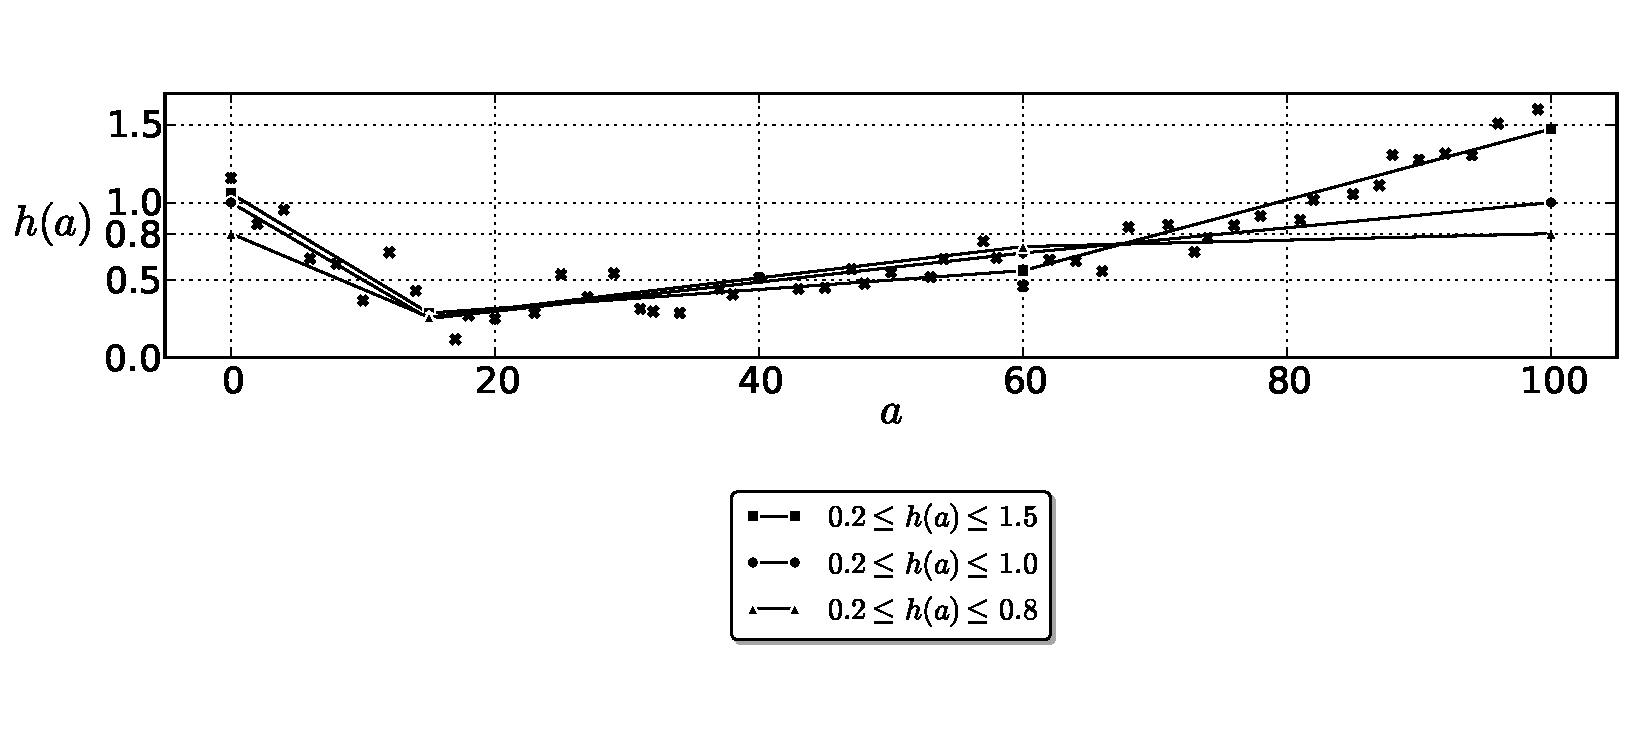
\includegraphics[width=\textwidth]{level_bound-smoothing-splines.pdf}
\caption{An informative prior on the upper and
lower bounds of $\mu(a)$ changes the estimated rate dramatically for
ages where the data is outside the bounds. For ages where the data is
inside the bounds, the estimates are also effected, but to a lesser
degree.}
\label{level-bounds-priors}
\end{center}
\end{figure}



Like the level value prior, this prior is also implemented as a
hard/soft constraint.  If the level bounds are $\ell_0 \leq \mu(a)
\leq \ell_1$, there is a hard part, that replaces the spline with a
clipped version, $\mu'(a) = \clip(\mu(a), \ell_0, \ell_1)$, and a
soft part that says that the original spline is close to the clipped
spline in offset-log-transformed space.

\section{Priors on monotonicity}

One common expert prior on age patterns is a strong belief that the
function is increasing or decreasing over a certain age
range. Mathematically speaking, these are priors on the sign of the
derivative of the age pattern.  This can be implemented efficiently in
Bayesian MCMC computation by conditioning on the differences of the
$\mu(a)$ in the age-pattern model, for example:
\[
\mu(a) \geq \mu(a+1) \text{for } a : a_s < a < a_e.
\]

The results of such a prior are shown in
Figure~\ref{monotone-age-pattern}.


\begin{figure}[h]
\begin{center}
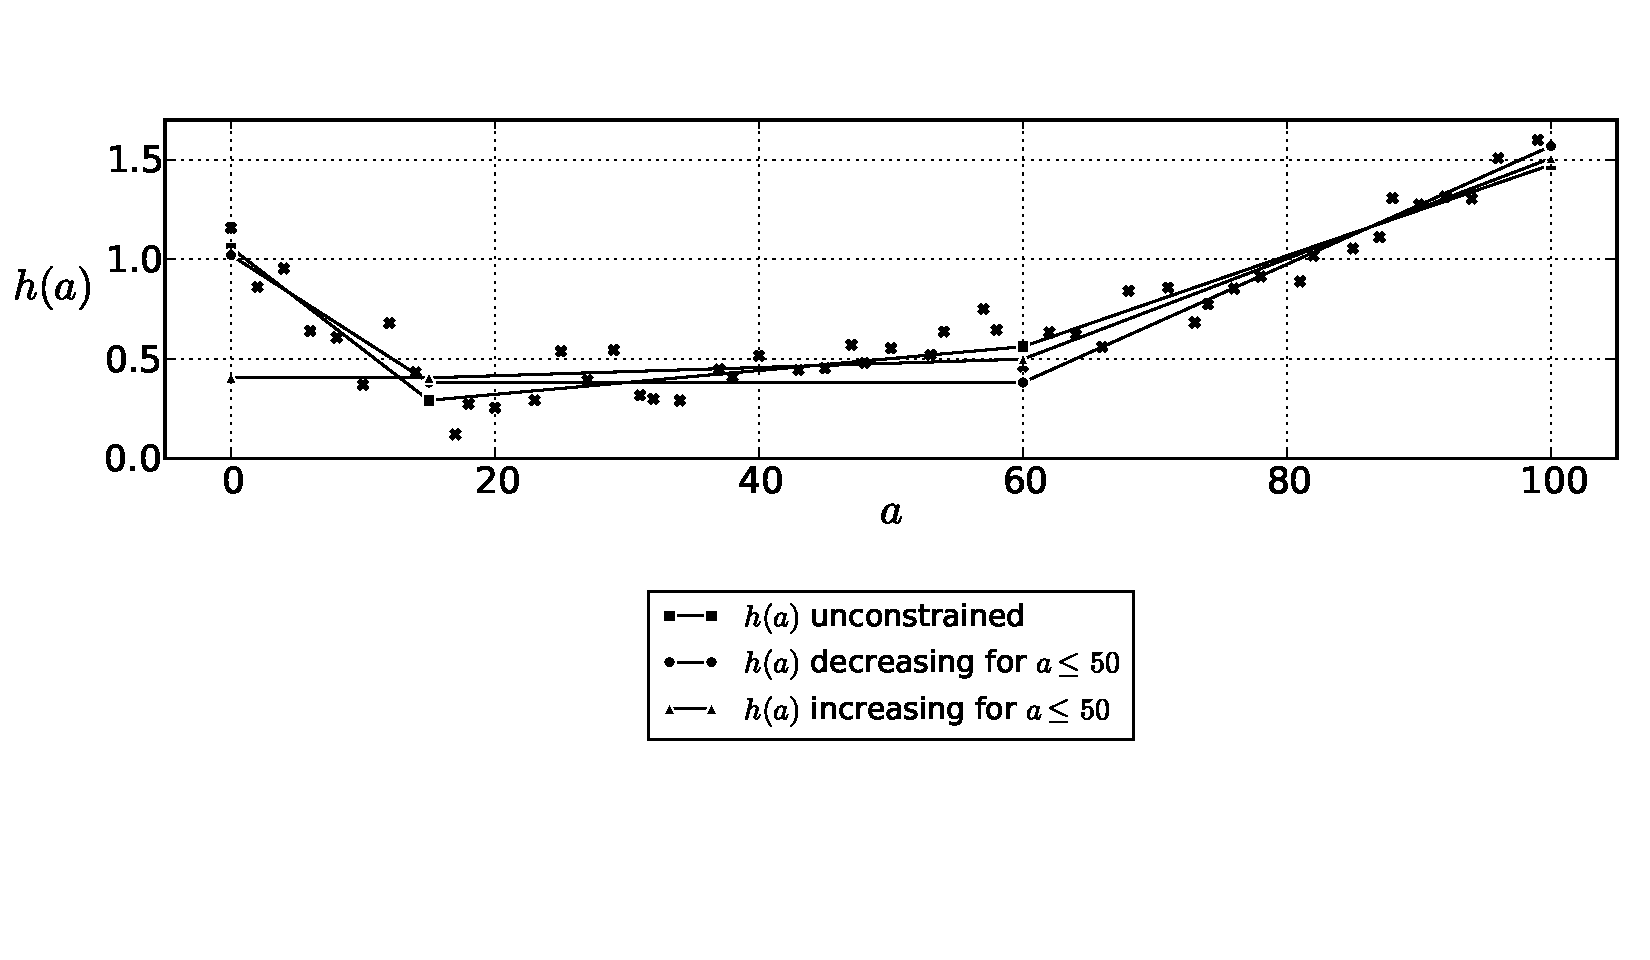
\includegraphics[width=\textwidth]{monotone-smoothing-splines.pdf}
\caption{The expert belief that the age pattern
is increasing or decreasing across an age range can also be
implemented as a Bayesian prior.  When the prior is contrary to the
data, for example the prior that $\mu(a)$ is increasing for $a \leq
50$ (shown as the line marked with triangles) with the data shown as
x-shaped markers which is clearly decreasing with age from 0 to 15,
the estimate will be as close to decreasing as possible, effectively
constant.}
\label{monotone-age-pattern}
\end{center}
\end{figure}


For computational efficiency, the increasing and decreasing
constraints are implemented as soft constraints.  For a constraint
that the function is decreasing between $a_s$ and $a_e$,
\[
\operatorname{clip}(\log \boldmu(a+1) - \log \boldmu(a), 0, 1) \sim \Normal(0, \epsilon^2),
\]
for a small value of $\epsilon$, like $\epsilon = 10^{-6}$.  This has
a fully Bayesian interpretation, saying that decreasing is expected
and an increase of more than around .0003\% is very surprising.


An area for future work comes from another common expert belief, that
the age pattern is unimodal.  This is conceptually clear, but
computationally it has proven more difficult to realize than
monotonicity.  While the monotonicity constraint maintains
log-concavity of the posterior distribution (if it was log-concave to
start with), a straightforward implementation of a unimodality
constraint will result in non-log-concave posterior distribution, even
if everything else is well behaved.  This suggests that the difficulty
in fitting such models in inherent in the local step method of the
MCMC algorithms I have been using.  Perhaps an alternative approach,
such as the population Monte Carlo algorithm would be more successful.
Alternatively, there are some approximations of the unimodality
constraint that may be easier to optimize over \cite{Papp[KP6]]}.

\section{Priors are not just for splines}
All three of the expert priors developed in this section are
applicable to any age-specific function derived from the compartmental
model in Section~\ref{compartmental-model}. Most importantly, the
age-specific prevalence $p = C/(S+C)$ can be augmented with expert
priors on level values (e.g. birth prevalence is zero), level bounds
(e.g. no population has prevalence above 10\%), and monotonicity
constraints (e.g. prevalence in increasing as a function of
age). Relative risk $\frac{m+f}{m}$ is another derived quantity that
experts often have strong priors about.

However, this sort of modeling requires care. The system dynamics
model enforces a precise consistency between the different
epidemiological rates, and making strong assumptions about one will
have implications for others.  Sometimes these implications are
counter-intuitive.

As a practical matter, I recommend modeling begin with as few
assumptions as possible, and gradually add in expert priors. The
benefit of this is threefold.  First, fitting the model without all of
the available expert knowledge allows the data to speak.  If it
confirms the expert belief that is reassuring, and if it shows the
opposite, that is interesting. Second, the MCMC algorithm has a
pitfall, \emph{non-convergence}. A quick way into this pit is
introducing inconsistent expert priors, for example decreasing
prevalence and prevalence of zero at age zero. By adding in expert
priors one at a time, the inconsistency that caused non-convergence
will be more easily identified. Third, as with any model that produces
estimates from sparse and noisy data, it is essential to conduct a
sensitivity analysis to understand how influential modeling
assumptions are on the results.  The gradual addition of expert priors
will provide a starting point for this sensitivity analysis, showing
which expert priors are essential to obtaining reasonable results, and
which are not as critical.

\section{Empirical priors on age patterns}
TK description of how to implement empirical priors on age patterns,
it's simple.  Just put informative prior on age-specific rate.
It's not just for splines, you can do it for anything.  Include
exact formulation that I ended up using (log-normal, I believe)
